\documentclass[oneside]{article}


% ------
% Fonts and typesetting settings
\usepackage[sc]{mathpazo}
\usepackage[T1]{fontenc}
\linespread{1.05} % Palatino needs more space between lines
\usepackage{microtype}


% ------
% Page layout
\usepackage[hmarginratio=1:1,top=32mm,columnsep=20pt]{geometry}
\usepackage[font=it]{caption}
\usepackage{paralist}
\usepackage{multicol}
\usepackage{amsmath}
% ------
% Lettrines
\usepackage{lettrine}


% ------
% Abstract
\usepackage{abstract}
	\renewcommand{\abstractnamefont}{\normalfont\bfseries}
	\renewcommand{\abstracttextfont}{\normalfont\small\itshape}


% ------
% Titling (section/subsection)
\usepackage{titlesec}
\renewcommand\thesection{\Roman{section}}
\titleformat{\section}[block]{\large\scshape\centering}{\thesection.}{1em}{}


% ------
% Header/footer
\usepackage{fancyhdr}
	\pagestyle{fancy}
	\fancyhead{}
	\fancyfoot{}
	\fancyhead[C]{Visión por Computador $\bullet$ 6 February 2016 $\bullet$ Universidad de Granada}
	\fancyfoot[RO,LE]{\thepage}


% ------
% Clickable URLs (optional)
\usepackage{hyperref}

% ------
% Maketitle metadata
\title{\vspace{-15mm}%
	\fontsize{24pt}{10pt}\selectfont
	\textbf{Fusión de imágenes con Poisson}
	}
\author{%
	\large
	\textsc{Alejandro Alcalde, Cristina Heredia}\thanks{Template by \href{http://www.howtotex.com}{howtoTeX.com}} \\[2mm]
	\normalsize	Universidad de Granada \\
	\normalsize	\href{mailto:frits@howtoTeX.com}{frits@howtoTeX.com}
	\vspace{-5mm}
	}
\date{}



%%%%%%%%%%%%%%%%%%%%%%%%
\usepackage{graphicx}
\begin{document}

\maketitle
\thispagestyle{fancy}

\begin{abstract}
\noindent Este trabajo corresponde al Proyecto final de la asignatura Visión por Computador y en él se aborda el problema de fusionar dos imágenes
distintas en una sola, intentando disimular que el resultado es una imágen artificial. Para ello, se desarrollan mecanismos de interpolación
basados en resolver ecuaciones de Poisson que nos permiten mezclar imágenes tanto opacas como no.
\end{abstract}


\lettrine[nindent=0em,lines=3]{E}n este proyecto nos centramos en la edición de imágenes a nivel local, ya que nuestro interés se centra en aplicar
cambios en una región seleccionada de una imágen concreta (imágen de destino) que normalmente implica incorporar la parte seleccionada de otra imágen
(imágen fuente)  a dicha imágen de destino en una posición indicada a voluntad, haciendo que dicha incorporación parezca lo más natural posible. \newline \newline Para lograr esto, hemos hecho una implementación
de algunas de las herramientas matemáticas que se describen en el papper \textbf{Poisson Image Editing}, concretamente, hemos implementado en código C++ la técnica de  \textbf{seamless Normal Clonning} y la de \textbf{Mixing Clonning} como una mejora alternativa
del anterior, ya que el empleo de mezcla de gradientes nos da mejores resultados con objetos con contenido transparente. \newline Para resolver el problema de la fusión de imágenes, en ambas implementaciones
se recurre, como aconseja el papper mencionado, a plantear y resolver tres ecuaciones de Poisson que hemos resuelto mediante descomposición de Cholesky. Una ecuación por cada canal de la imágen( pues hemos trabajado en espacio RGB), que finalmente se usarán
para obtener la imágen final. \newline

\section{Procedimiento y Solución de Poisson}

La técnica de Poisson resuelve el problema definido como: \[min_{I}\int \int_{}^{\Omega } \parallel \bigtriangledown I-V\parallel^{2}\] con \[I|\partial_{\Omega}=I^{*}\], donde
I es la imágen objetivo, \[\bigtriangledown =\left [\frac{\partial }{\partial x},\frac{\partial }{\partial y} \right ]\]
es el operador de gradiente y V es el guidance field. Su solución es la única solución a la siguiente ecuación de Poisson: \newline
$\Delta I=div V$ con $I|\partial_{\Omega}=I^{*}$ donde $\Delta=\frac{\partial^2 }{\partial x^2}+\frac{\partial^2 }{\partial y^2}$ es el operador
Laplaciano y $div=\frac{\partial }{\partial x}+\frac{\partial }{\partial y}$ es el operador de divergencia. \newline
Así pues nosotros necesitaremos resolver tres ecuaciones de la forma anterior, una para cada canal de la imagen(RGB). \newline
Esto en forma matricial y discretizada, equivaldrá a resolver tres ecuaciones de la forma $Ax=b$ por lo que el vector $x$ será $x=A\setminus b$ o equivalentemente $x=A ^{-1}*b$, donde A denota la matriz de coefficientes y b será el Vector solución. \newline
La matriz de Coefficientes, que contendrá 0, -1 o 4 si pertenece a la diagonal, representará un núcleo de convolución ya que los píxeles estarán influenciados
por sus cuatro vecinos adyacentes. \newline
El vector Solución, b, tendrá tres filas, una por cada color de la imágen, y se obtiene resolviendo:
\[\mid N_{p} \mid f_{p}-\sum_{q\epsilon N_{p}\bigcap \Omega} f_{q}=\sum_{q\epsilon N_{p}\bigcap \partial\Omega}f^{*}_{q}+\sum_{q\epsilon N_{p}}v_{pq}\]
para cada $ p \epsilon \Omega$, donde $\Omega$ denota los píxeles blancos de la imágen máscara, f es una función desconocida definida en el interior de $\Omega$
q es calquier pixel vecino de p ($q \epsilon N_{p}$) y $v_{pq}$ es el gradiente (guidance field o guidance vect), que en función del método
se calculará de una manera o de otra. \newline

\section{Seamless Normal Cloning}
Como hemos mencionado, hemos implementado dos soluciones al problema. La primera de ellas fue el Seamless Normal Clonning.
Ahora que sabemos la parte común a los dos métodos, veamos cómo se obtiene el guidance vect, que es la parte que difiere. \newline
El método más básico se basa en importar los gradientes directamente de la imágen fuente (imágen que queremos copiar en otra), esto es:
Siendo $g$ la imágen fuente, $v= \bigtriangledown g $ ahora las ecuaciones a resolver serían de la forma:
$\Delta f=\Delta g$  sobre $\Omega$, con $f\mid_{\partial \Omega}=f^{*}\mid_{\partial\Omega}$ donde $f$ se define sobre $\Omega$ (región blanca de la máscara)
y $f^{*}$ de define sobre el complementode $\Omega$ (región negra). \newline
Computacionalmente, se calcula como: \newline
para todo $<p,q>,v_{pq} =g_{p}-g_{q}$ donde $<p,q>$ son parejas de píxees vecinos. Para cada uno de los canales de la imágen. \newline
No da malos resultados, pero con imágenes con algo de transparencia, como una nube por ejemplo, no funciona del todo bien.

\section{Seamless Mixing Cloning}
Ésta es una implementación mejorada del Seamless Normal Cloning, cuando se quieren copiar imágenes con algún contenido transparente.
A diferencia del método anterior, aquí se calcula el guidance Vect tomando el gradiente más fuerte entre la imágen fuente y la imágen de destino.
En forma discretizada: \newline
\[v_{pq}=\left\{\begin{matrix} f^{*}_{p}-f^{*}_{q} if \mid f^{*}_{p}-f^{*}_{q}\mid > \mid g_{p}-g_{q} \mid \\ g_{p}-g_{q} \end{matrix}\right.\]

que indica que $v_{pq}$ será $g_{p}-g_{q}$ en otro caso(si no se cumple el anterior).


\begin{figure}[htbp]
\centering
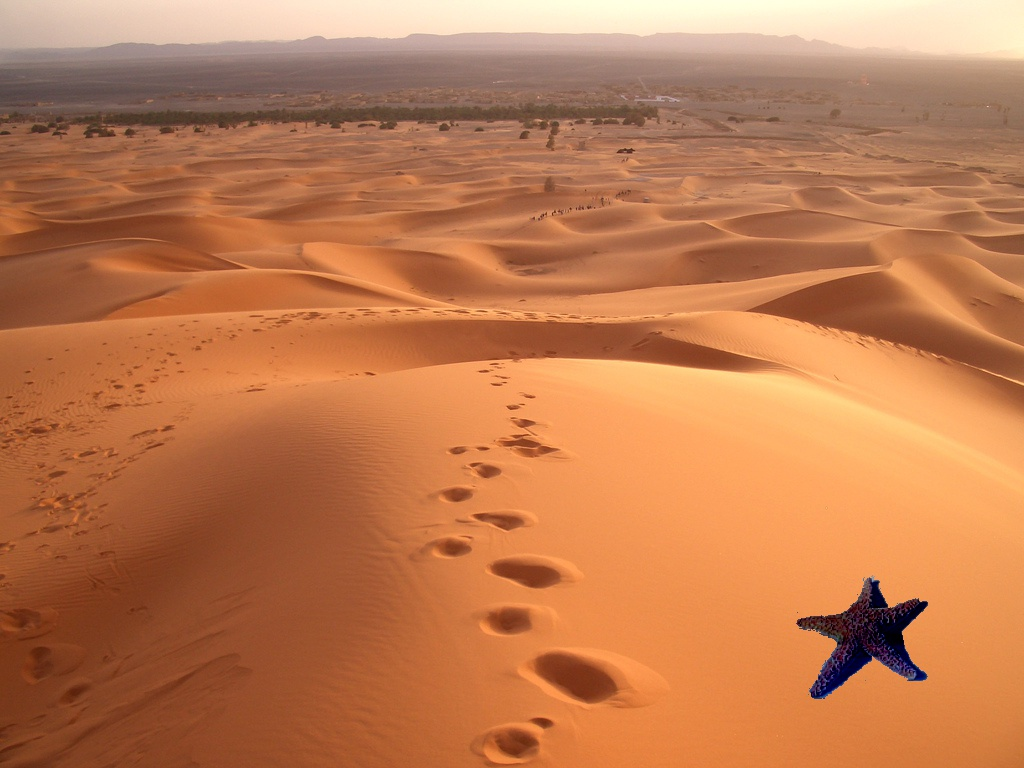
\includegraphics[width=1\textwidth]{./img/mix_dest_desert_estrella}
\caption{}
\label{fig:1}
\end{figure}

\begin{figure}[htbp]
\centering
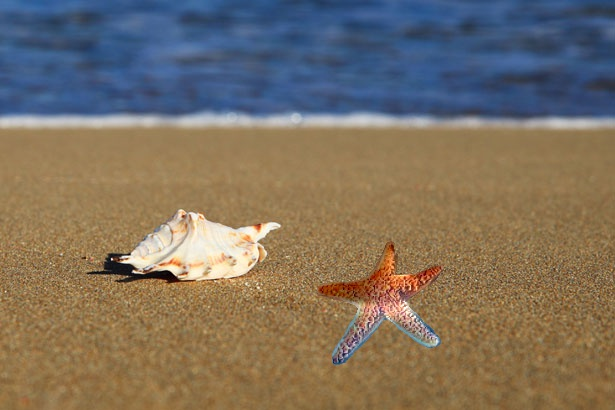
\includegraphics[width=1\textwidth]{./img/mix_dest_sand_estrella2.jpg}
\caption{}
\label{fig:2}
\end{figure}

\begin{figure}[htbp]
\centering
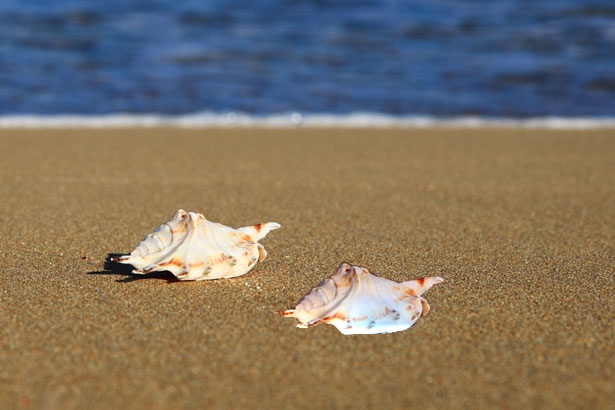
\includegraphics[width=1\textwidth]{./img/mix_dest_sand_shell2.jpg}
\caption{}
\label{fig:3}
\end{figure}

\begin{figure}[htbp]
\centering
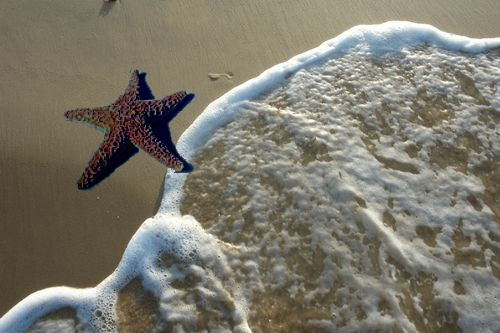
\includegraphics[width=1\textwidth]{./img/mix_dest_water_estrella.jpg}
\caption{}
\label{fig:4}
\end{figure}

\begin{figure}[htbp]
\centering
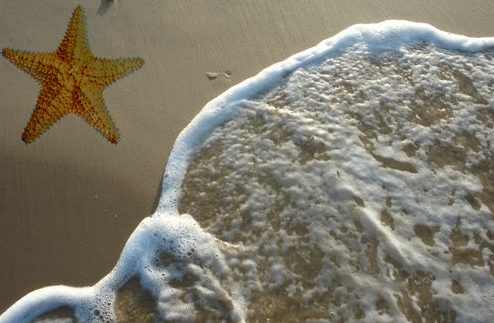
\includegraphics[width=.5\textwidth]{./img/mix_Mixing_starSea.png}
\caption{}
\label{fig:5}
\end{figure}


\begin{figure}[htbp]
\centering
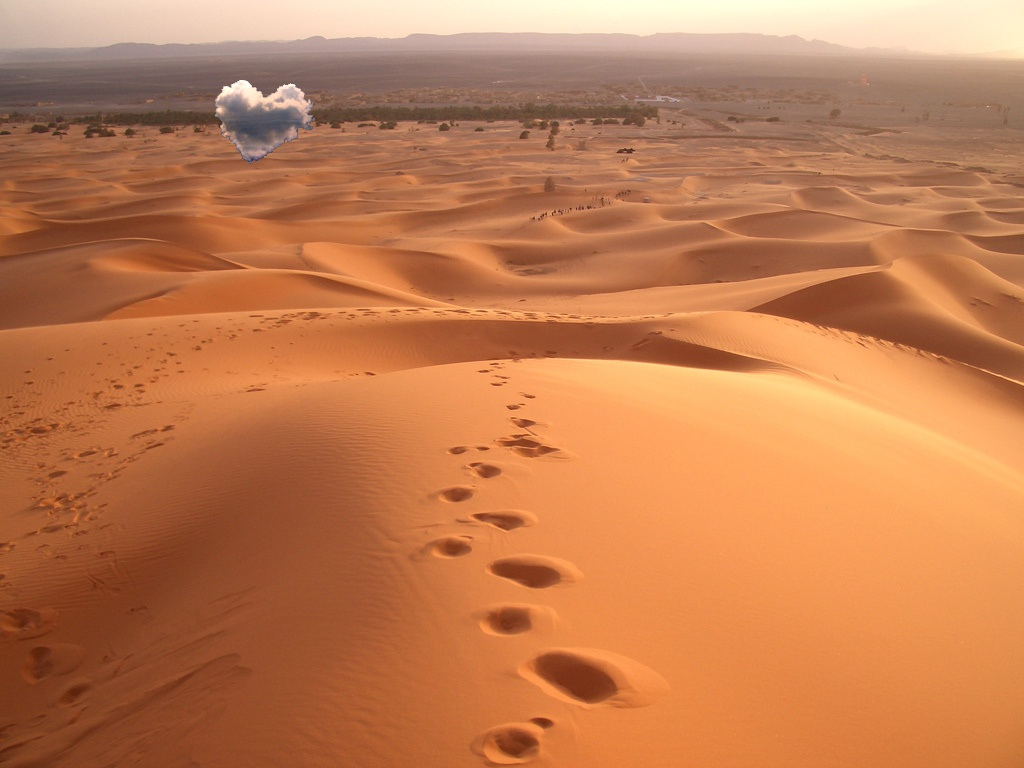
\includegraphics[width=1\textwidth]{./img/mix_dest_desert_nube.jpg}
\caption{}
\label{fig:6}
\end{figure}

\begin{figure}[htbp]
\centering
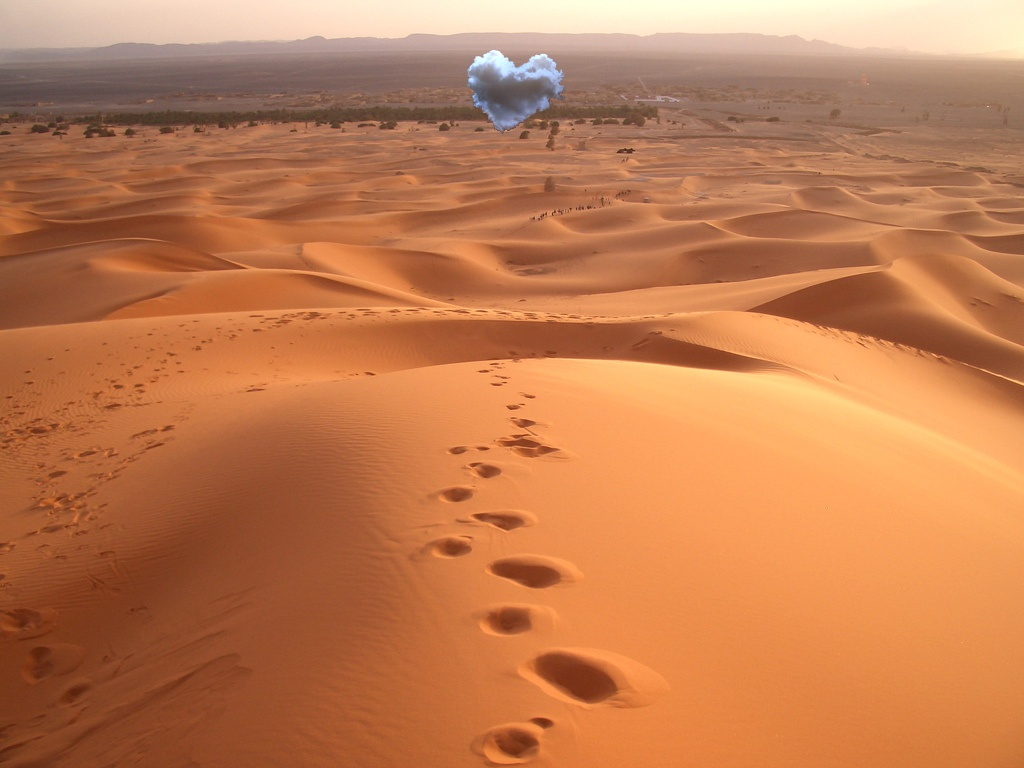
\includegraphics[width=1\textwidth]{./img/normal_dest_desert_nube.jpg}
\caption{}
\label{fig:7}
\end{figure}

\begin{figure}[htbp]
\centering
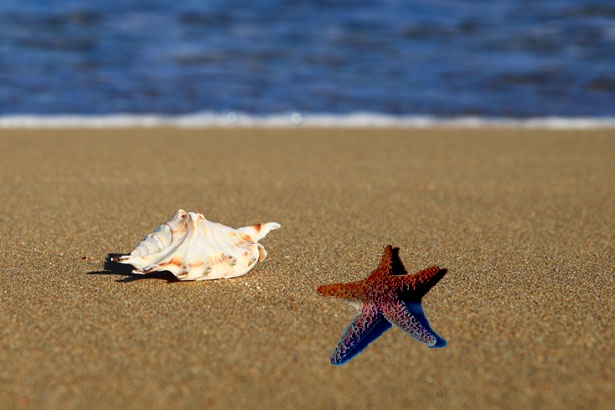
\includegraphics[width=1\textwidth]{./img/mix_dest_sand_estrella.jpg}
\caption{}
\label{fig:8}
\end{figure}

\begin{figure}[htbp]
\centering
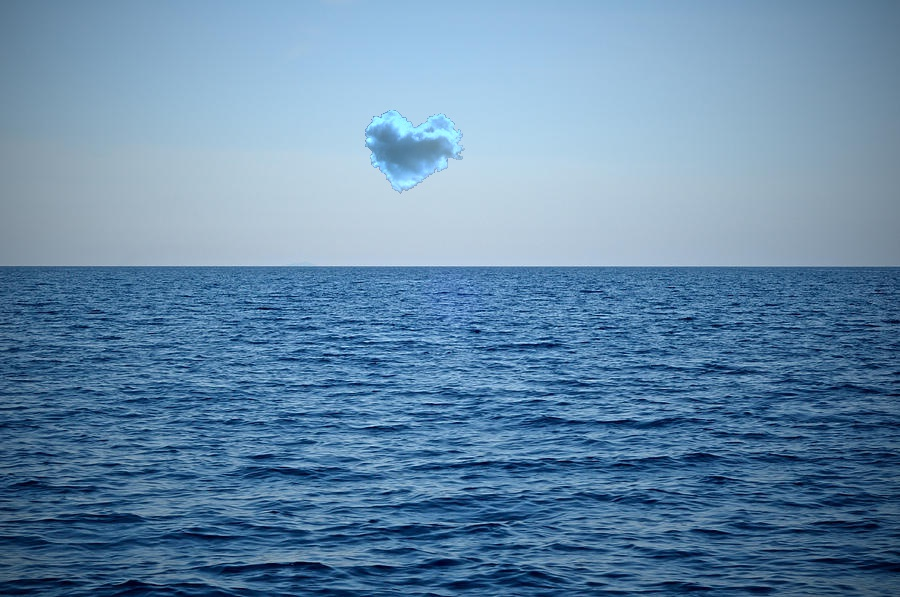
\includegraphics[width=1\textwidth]{./img/mix_dest_sea_nube.jpg}
\caption{}
\label{fig:9}
\end{figure}

\begin{figure}[htbp]
\centering
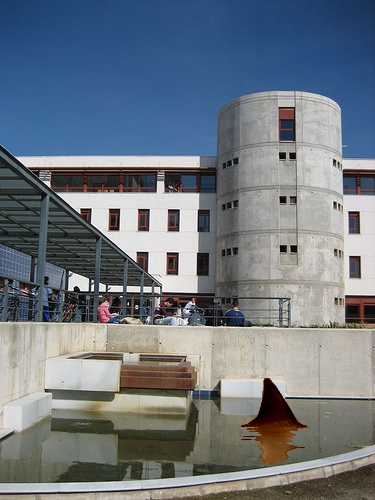
\includegraphics[width=1\textwidth]{./img/mix_etsiit_aleta.jpg}
\caption{}
\label{fig:10}
\end{figure}

\begin{figure}[htbp]
\centering
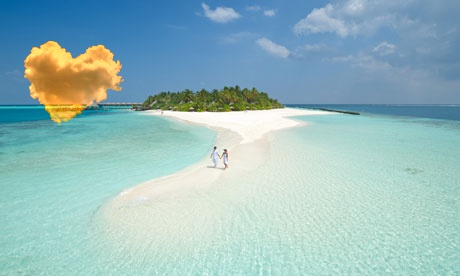
\includegraphics[width=1\textwidth]{./img/mix_nubebn1mixed.jpg}
\caption{}
\label{fig:11}
\end{figure}


\bibliography{biblio}{}
\bibliographystyle{IEEEtran}

\nocite{*}

\end{document}